\subsection{Explicit upwind scheme parallel algorithm} \label{s:general-approach:explicit-upwind-parallel-algorithm}
	Dependency of the explicit upwind scheme is presented in Figure \ref{fig:stencil:explicit-upwind}. According to the \gls{stencil} in order to calculate new point at time $n+1$ this scheme requires previous and current point of a grid from time $n$. It means that each of the processors requires one value from previous processor (in terms of their ids) to start calculations. Figure \ref{fig:communication:explicit-upwind} presents discussed earlier communication between processors. Transfered $f_{lmax}^{n}$ relates to the last point in the local grid, where $lmax$ is calculated as shown in Listing \ref{lst:fragmentation}.
	\begin{figure}[!htbp]
		\centering
		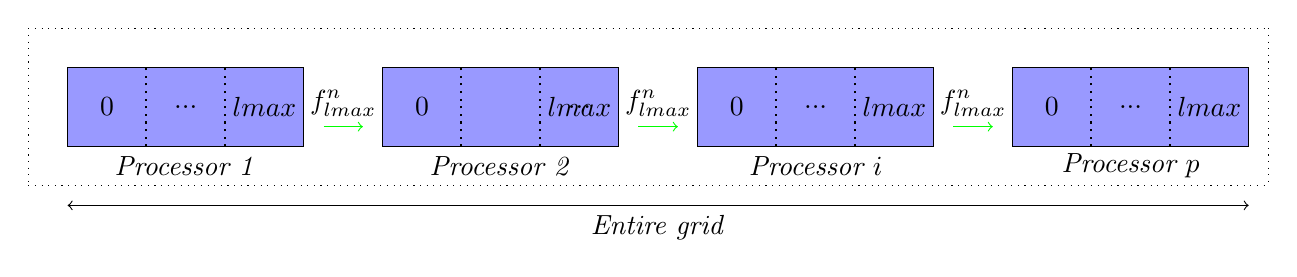
\begin{tikzpicture}[scale=1.0]
			\draw[dotted] (-0.5,-0.5) -- (15.25,-0.5);
			\draw[dotted] (-0.5, 1.5) -- (15.25, 1.5);
			\draw[dotted] (-0.5, 1.5) -- (-0.5, -0.5);
			\draw[dotted] (15.25, 1.5) -- (15.25, -0.5);
			
			\filldraw[fill=blue!40!white, draw=black] (0,0) rectangle (3,1);
			\node[black] at (0.5,0.5) {$0$};
			\draw[black, dotted, line width = 0.75pt] (1, 0) -- (1, 1);
			\node[black] at (1.5,0.5) {...};
			\draw[black, dotted, line width = 0.75pt] (2, 0) -- (2, 1);
			\node[black] at (2.5,0.5) {$lmax$};
			
			\filldraw[fill=blue!40!white, draw=black] (4,0) rectangle (7,1);
			\node[black] at (4.5,0.5) {$0$};
			\draw[black, dotted, line width = 0.75pt] (5, 0) -- (5, 1);
			\node[black] at (6.5,0.5) {...};
			\draw[black, dotted, line width = 0.75pt] (6, 0) -- (6, 1);
			\node[black] at (6.5,0.5) {$lmax$};
			
			\filldraw[fill=blue!40!white, draw=black] (8,0) rectangle (11,1);
			\node[black] at (8.5,0.5) {$0$};
			\draw[black, dotted, line width = 0.75pt] (9, 0) -- (9, 1);
			\node[black] at (9.5,0.5) {...};
			\draw[black, dotted, line width = 0.75pt] (10, 0) -- (10, 1);
			\node[black] at (10.5,0.5) {$lmax$};
			
			\filldraw[fill=blue!40!white, draw=black] (12,0) rectangle (15,1);
			\node[black] at (12.5,0.5) {$0$};
			\draw[black, dotted, line width = 0.75pt] (13, 0) -- (13, 1);
			\node[black] at (13.5,0.5) {...};
			\draw[black, dotted, line width = 0.75pt] (14, 0) -- (14, 1);
			\node[black] at (14.5,0.5) {$lmax$};
			
			\node[align=right] at (1.5, -0.25) {\emph{Processor 1}};
			\node[align=right] at (5.5, -0.25) {\emph{Processor 2}};
			\node[align=right] at (9.5, -0.25) {\emph{Processor $i$}};
			\node[align=right] at (13.5, -0.25) {\emph{Processor $p$}};
			\draw [->][green] (3.25, 0.25) -- node [midway, above, sloped, black] {$f_{lmax}^{n}$} (3.75, 0.25);
			\draw [->][green] (7.25, 0.25) -- node [midway, above, sloped, black] {$f_{lmax}^{n}$} (7.75, 0.25);
			\draw [->][green] (11.25, 0.25) -- node [midway, above, sloped, black] {$f_{lmax}^{n}$} (11.75, 0.25);
			\draw[<->] (0,-0.75) -- node [midway, below, sloped, black] {\emph{Entire grid}} (15,-0.75);
		\end{tikzpicture}
		\caption{Communication between processors in parallel explicit upwind schema.}
		\label{fig:communication:explicit-upwind}
	\end{figure}
	Parallel calculations for explicit upwind schema are visualized in Figure \ref{fig:visualization:explicit-upwind}. This scheme depends only on current solution so boundary values can be send between neighboring processors before each full iteration through local grids. We can assume that all the processors will be working simultaneously with a small advantage of first processor, because it doesn't have to receive boundary condition. 
	\begin{figure}[!htbp]
		\centering
		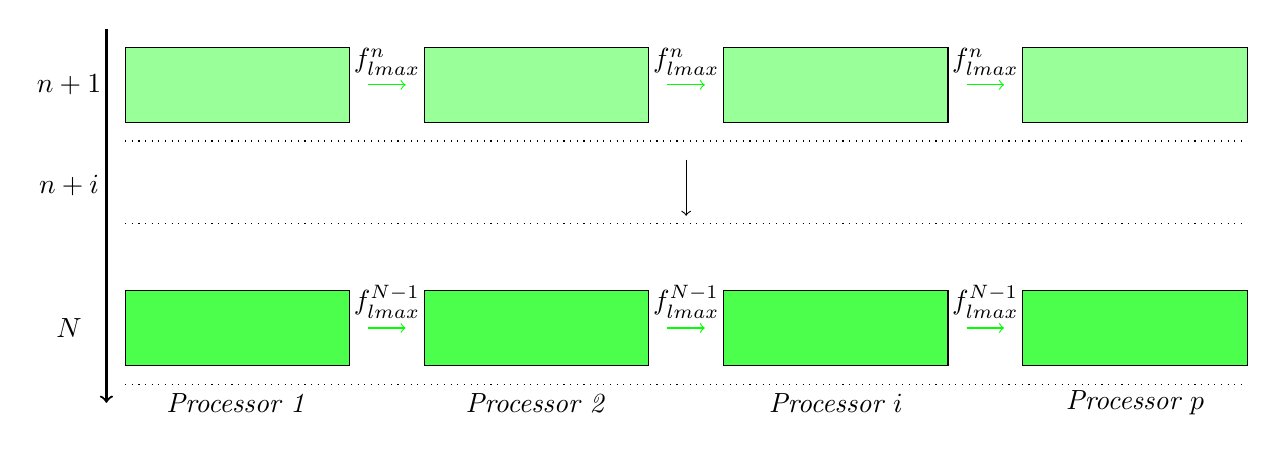
\begin{tikzpicture}[scale=0.95]
			\draw [->] [black, thick] (-.25, 0.25) -- (-.25, -4.75);
			\node[black] at (-0.75, -0.5) {$n+1$};
			\draw [->][green] (3.25, -.5) -- node [midway, above, sloped, black] {$f_{lmax}^{n}$} (3.75, -.5);
			\draw [->][green] (7.25, -.5) -- node [midway, above, sloped, black] {$f_{lmax}^{n}$} (7.75, -.5);
			\draw [->][green] (11.25, -.5) -- node [midway, above, sloped, black] {$f_{lmax}^{n}$} (11.75, -.5);
			\filldraw[fill=green!40!white, draw=black] (0,0) rectangle (3,-1);
			\filldraw[fill=green!40!white, draw=black] (4,0) rectangle (7,-1);
			\filldraw[fill=green!40!white, draw=black] (8,0) rectangle (11,-1);
			\filldraw[fill=green!40!white, draw=black] (12,0) rectangle (15,-1);
			
			\draw [dotted] (0,-1.25) -- (15,-1.25);			
			\draw [->] [black] (7.5, -1.5) -- (7.5, -2.25);
			\draw [dotted] (0,-2.35) -- (15,-2.35);
			
			\node[black] at (-0.75, -1.85) {$n + i$};
			
			\node[black] at (-0.75, -3.75) {$N$};
			\draw [->][green] (3.25, -3.75) -- node [midway, above, sloped, black] {$f_{lmax}^{N -1}$} (3.75, -3.75);
			\draw [->][green] (7.25, -3.75) -- node [midway, above, sloped, black] {$f_{lmax}^{N -1}$} (7.75, -3.75);
			\draw [->][green] (11.25, -3.75) -- node [midway, above, sloped, black] {$f_{lmax}^{N -1}$} (11.75, -3.75);
			\filldraw[fill=green!70!white, draw=black] (0,-3.25) rectangle (3,-4.25);
			\filldraw[fill=green!70!white, draw=black] (4,-3.25) rectangle (7,-4.25);
			\filldraw[fill=green!70!white, draw=black] (8,-3.25) rectangle (11,-4.25);
			\filldraw[fill=green!70!white, draw=black] (12,-3.25) rectangle (15,-4.25);
			\draw [dotted] (0,-4.5) -- (15,-4.5);
			
			\node[align=right] at (1.5, -4.75) {\emph{Processor 1}};
			\node[align=right] at (5.5, -4.75) {\emph{Processor 2}};
			\node[align=right] at (9.5, -4.75) {\emph{Processor $i$}};
			\node[align=right] at (13.5, -4.75) {\emph{Processor $p$}};
			
		\end{tikzpicture}
		\caption{Visualization of parallel calculations for explicit upwind scheme.}
		\label{fig:visualization:explicit-upwind}
	\end{figure}